\section{(Model-based Goal-based) Utility-based Agents}\label{AI: Agent Programs/(Model-based Goal-based) Utility-based Agents}


\begin{figure}[H]
    \centering
    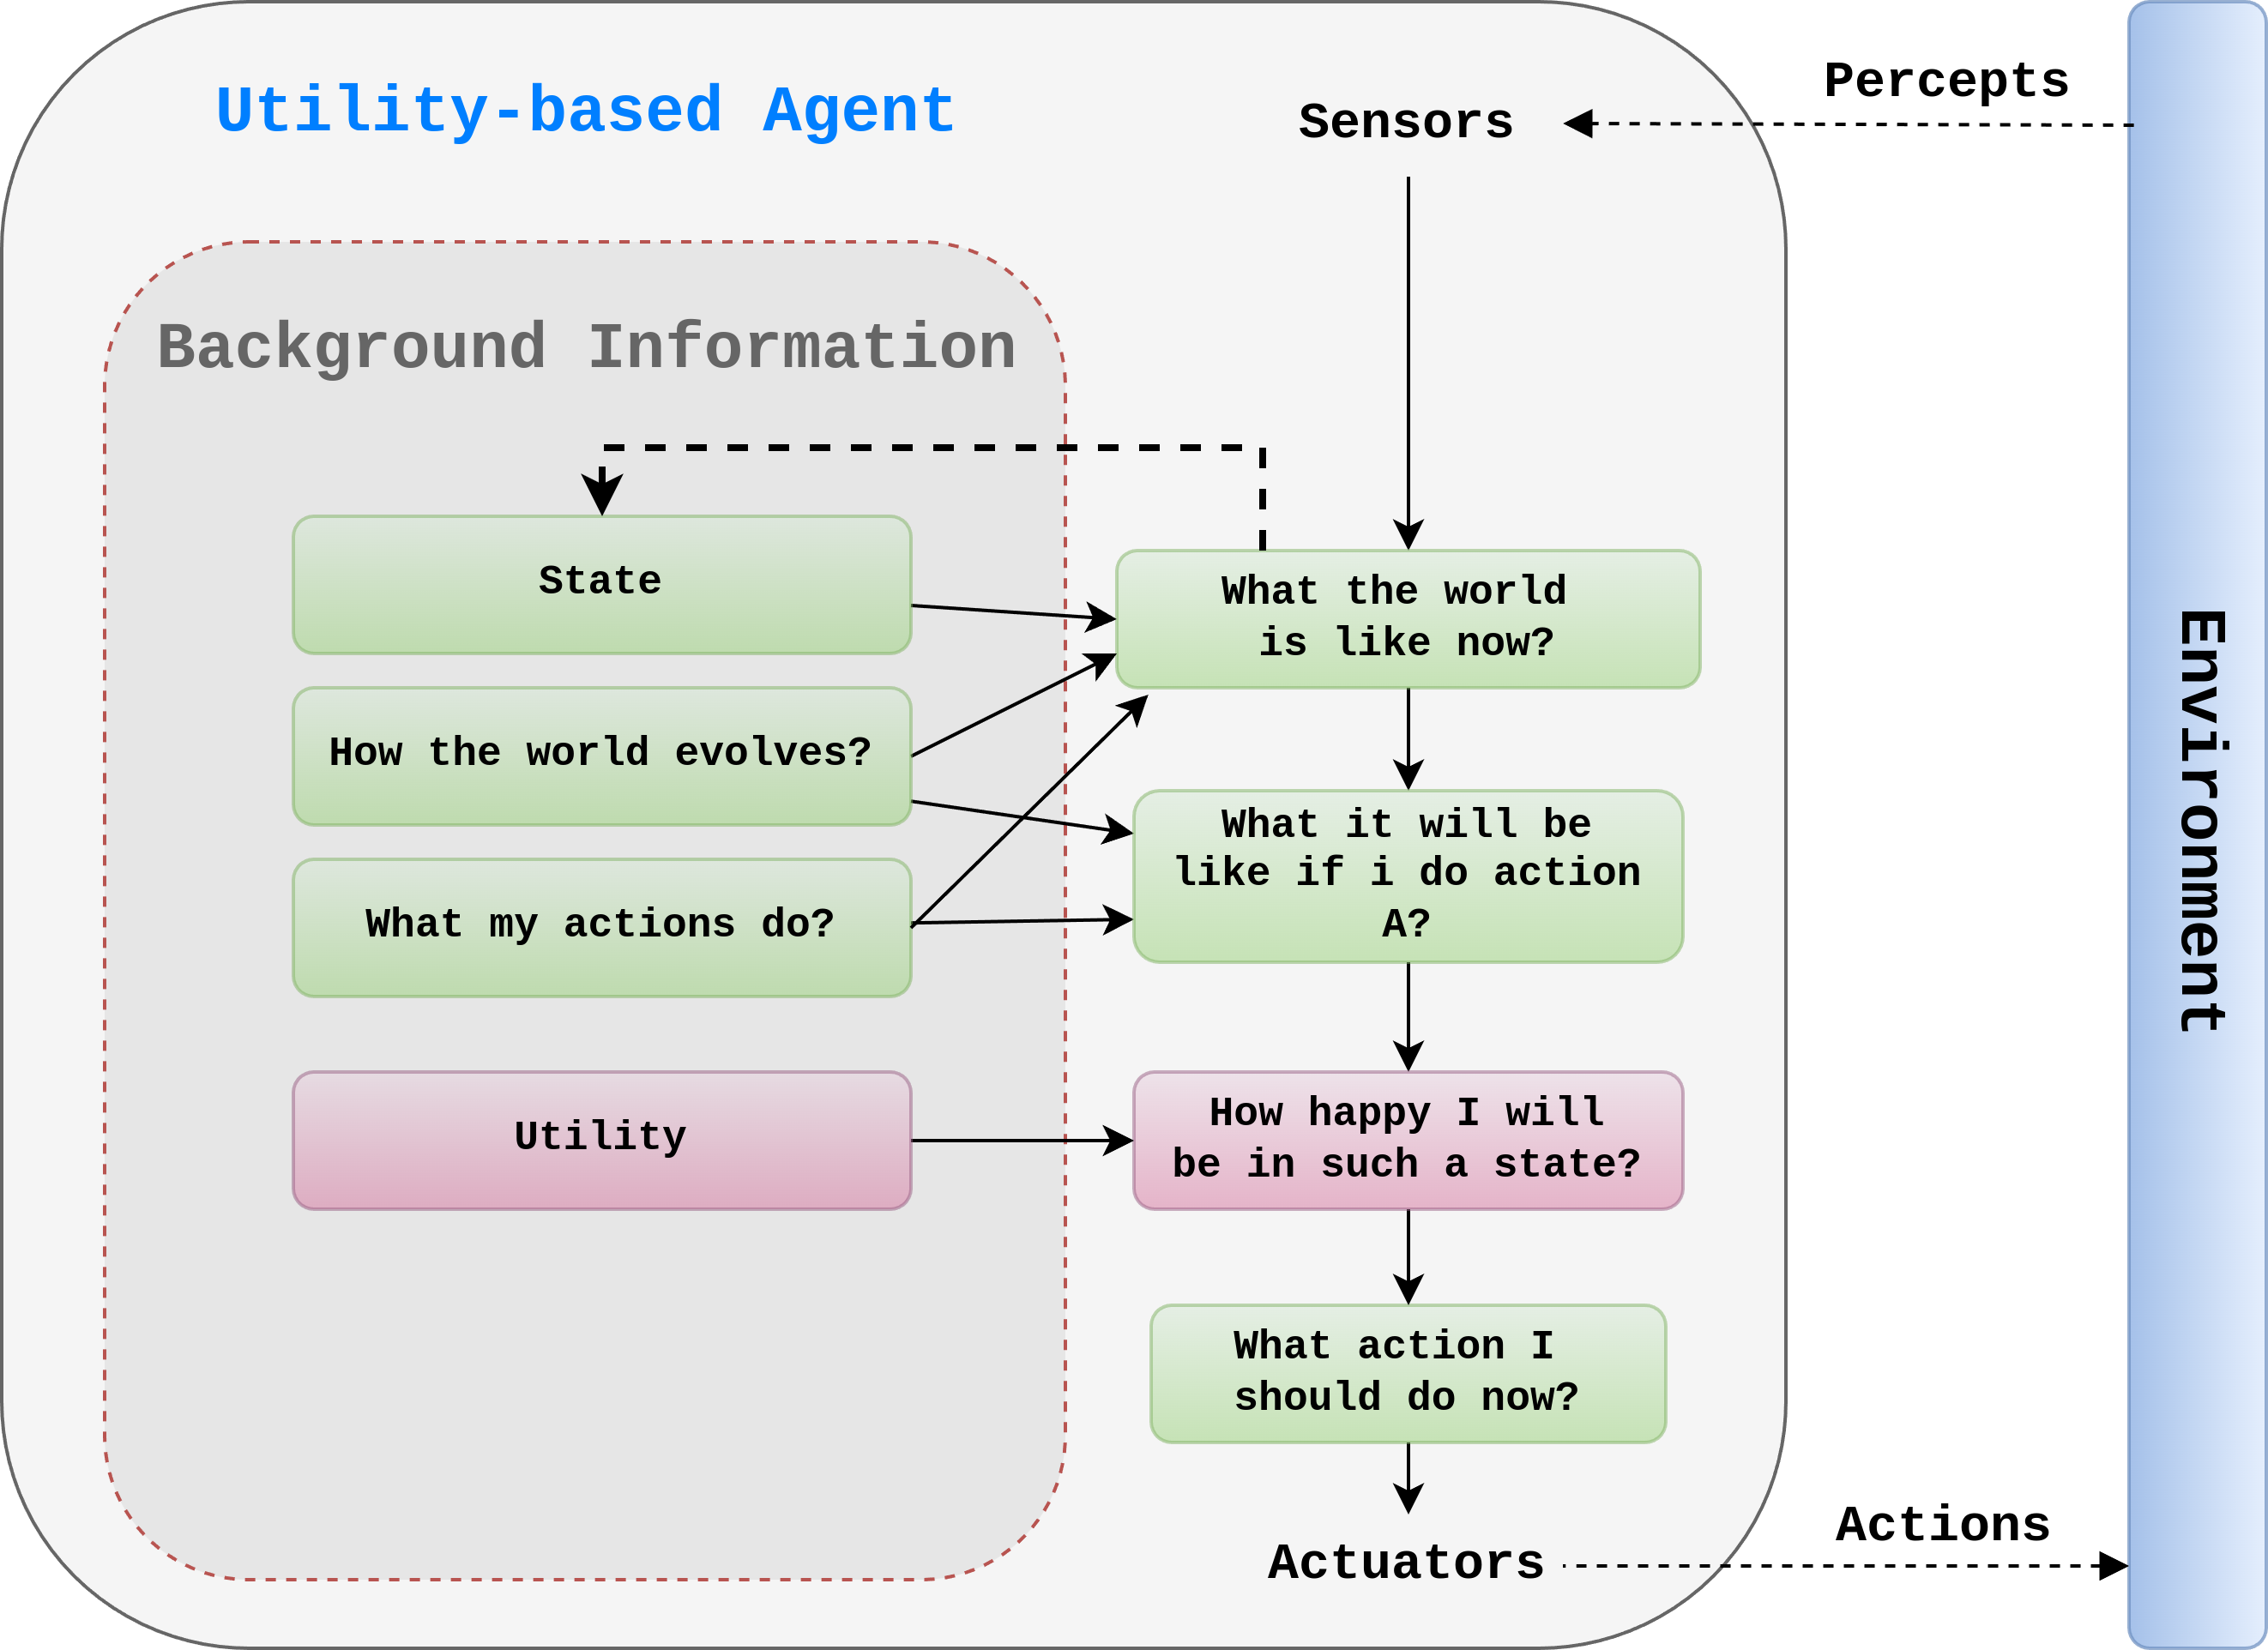
\includegraphics[
        width=0.5\linewidth, 
        height=6cm, 
        keepaspectratio
    ]{images/artificial-intelligence/ai-agents/agents-utility-based-agent.png}
    \caption*{A model-based, goal-based, utility-based agent. \cite{common/online/tools/draw.io}}
\end{figure}

\hspace{0.5cm}

\begin{enumerate}
    \item A more general performance measure than Goal (happy/ unhappy) should allow a comparison of different world states according to exactly how happy they would make the agent.
    \hfill \cite{ai/book/Artificial-Intelligence-A-Modern-Approach/Russell-Norvig}

    \item An agent’s \textbf{utility function} is essentially an internalization of the performance measure. 
    \hfill \cite{ai/book/Artificial-Intelligence-A-Modern-Approach/Russell-Norvig}
    \\
    (The word “utility” here refers to “\textit{the quality of being useful}”)

    \item  If the internal utility function and the external performance measure are in agreement, then an agent that chooses actions to maximize its utility will be rational according to the external performance measure.
    \hfill \cite{ai/book/Artificial-Intelligence-A-Modern-Approach/Russell-Norvig}

    \item this is \textbf{not the only} way to be rational but, like goal-based agents, a utility-based agent has many advantages in terms of flexibility and learning
    \hfill \cite{ai/book/Artificial-Intelligence-A-Modern-Approach/Russell-Norvig}

    \item (\textbf{Advantage}) in two kinds of cases, goals are inadequate but a utility-based agent can still make rational decisions:
    \begin{enumerate}
        \item when there are conflicting goals, only some of which can be achieved (for example, speed and safety), the utility function specifies the appropriate tradeoff
        \hfill \cite{ai/book/Artificial-Intelligence-A-Modern-Approach/Russell-Norvig}

        \item when there are several goals that the agent can aim for, none of which can be achieved with certainty, utility provides a way in which the likelihood of success can be weighed against the importance of the goals.
        \hfill \cite{ai/book/Artificial-Intelligence-A-Modern-Approach/Russell-Norvig}
    \end{enumerate}

    \item Partial observability and stochasticity are ubiquitous in the real world, and so, therefore, is decision making under uncertainty. 
    \hfill \cite{ai/book/Artificial-Intelligence-A-Modern-Approach/Russell-Norvig}

    \item a rational utility-based agent chooses the action that maximizes the expected utility of the action outcomes - that is, the utility the agent expects to derive, on average, given the probabilities and utilities of each outcome.
    \hfill \cite{ai/book/Artificial-Intelligence-A-Modern-Approach/Russell-Norvig}

    \item An agent that possesses an explicit utility function can make rational decisions with a general-purpose algorithm that does not depend on the specific utility function being maximized. In this way, the “global” definition of rationality - designating as rational those agent functions that have the highest performance - is turned into a “local” constraint on rational-agent designs that can be expressed in a simple program.
    \hfill \cite{ai/book/Artificial-Intelligence-A-Modern-Approach/Russell-Norvig}

    \item A utility-based agent has to model and keep track of its environment, tasks that have involved a great deal of research on perception, representation, reasoning, and learning.
    \hfill \cite{ai/book/Artificial-Intelligence-A-Modern-Approach/Russell-Norvig}

    \item Choosing the utility-maximizing course of action is also a difficult task, requiring ingenious algorithms.
    \hfill \cite{ai/book/Artificial-Intelligence-A-Modern-Approach/Russell-Norvig}
\end{enumerate}



\vspace{0.5cm}


\begin{customArrayStretch}{1.3}
\begin{table}[H]
\centering

\begin{tabular}{| l | l | l |}

\hline

\textbf{Aspect} & 
    \textbf{Utility Function} & 
    \textbf{Performance Measure} \\ \hline
    
\textbf{Perspective} & 
    From the agent’s point of view & 
    From the external evaluator’s point of view \\ \hline

\textbf{Goal} & 
    Maximize expected utility & 
    Maximize measurable performance \\ \hline

\textbf{Usage} & 
    Guides decision-making & 
    Evaluates overall system success \\ \hline

\end{tabular}

\caption*{Utility Function VS Performance Measure}
\end{table}
\end{customArrayStretch}














